\documentclass[10pt]{article}
\usepackage{amsmath,amsfonts,times}
\usepackage{graphicx,color,tikz}
\usepackage[paperwidth=17.6cm,paperheight=11.0cm,lmargin=0in,rmargin=0in,tmargin=0.in,bmargin=0.in]{geometry}
\usepackage{bm}
\usetikzlibrary{arrows.meta,calc,positioning}

% A box with a ball cut out of it, traced along a ray from its parts' spans: each part's spans (where the ray
% is inside it), the complement's, and the difference's, with its first crossing.
\definecolor{cray}{rgb}{0.10,0.35,0.80}
\definecolor{cbox}{rgb}{0.05,0.55,0.20}
\definecolor{cball}{rgb}{0.50,0.20,0.65}
\definecolor{cresult}{rgb}{0.90,0.50,0.00}
\definecolor{chit}{rgb}{0.80,0.10,0.10}
\definecolor{csolid}{rgb}{0.78,0.78,0.80}

\tikzset{
  ray/.style={-{Stealth[length=2.5mm]}, line width=1.1pt, draw=cray},
  span/.style={line width=4pt},
  crossing/.style={circle, fill=black, inner sep=0pt, minimum width=5pt},
  open/.style={circle, draw=black, fill=white, thick, inner sep=0pt, minimum width=5pt},
  rowlabel/.style={font=\small, anchor=east, align=right},
  note/.style={font=\scriptsize, align=left},
  guide/.style={black!25, densely dotted},
}

\begin{document}
\nopagecolor
\centering
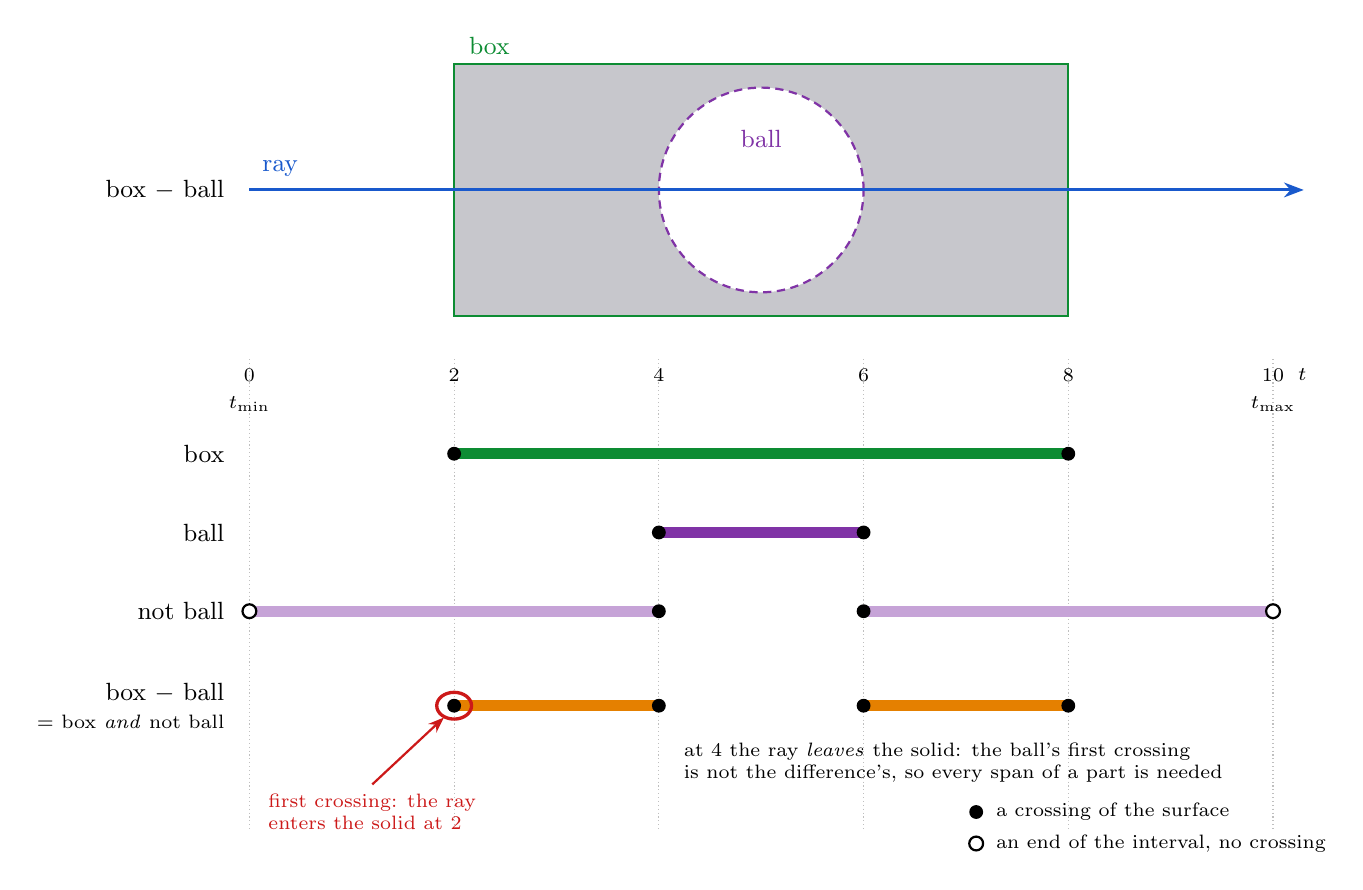
\begin{tikzpicture}[x=1.3cm, y=1cm]

  % ── The object along the ray: a box over [2, 8] with a ball over [4, 6] cut out of it.
  \begin{scope}[shift={(0,0.55)}]
    \fill[csolid] (2,-1.6) rectangle (8,1.6);
    \fill[white] (5,0) circle[radius=1.3cm];
    \draw[thick, cbox] (2,-1.6) rectangle (8,1.6);
    \draw[thick, cball, densely dashed] (5,0) circle[radius=1.3cm];
    \node[font=\small, text=cbox, anchor=south west] at (2.05,1.6) {box};
    \node[font=\small, text=cball] at (5,0.65) {ball};
    \draw[ray] (0,0) -- (10.3,0);
    \node[font=\small, text=cray, anchor=south] at (0.3,0.05) {ray};
    \node[rowlabel] at (-0.15,0) {box $-$ ball};
  \end{scope}

  % Distances along the ray, shared by every row below.
  \foreach \t in {0,2,4,6,8,10} {
    \draw[guide] (\t,-1.6) -- (\t,-7.6);
    \node[font=\scriptsize] at (\t,-1.8) {$\t$};
  }
  \node[font=\scriptsize, anchor=west] at (10.15,-1.8) {$t$};
  \node[font=\scriptsize, anchor=north] at (0,-1.95) {$t_\mathrm{min}$};
  \node[font=\scriptsize, anchor=north] at (10,-1.95) {$t_\mathrm{max}$};

  % ── Each part's spans.
  \node[rowlabel] at (-0.15,-2.8) {box};
  \draw[span, cbox] (2,-2.8) -- (8,-2.8);
  \node[crossing] at (2,-2.8) {}; \node[crossing] at (8,-2.8) {};

  \node[rowlabel] at (-0.15,-3.8) {ball};
  \draw[span, cball] (4,-3.8) -- (6,-3.8);
  \node[crossing] at (4,-3.8) {}; \node[crossing] at (6,-3.8) {};

  % ── The complement: the gaps, ending where the interval ends (no crossing there).
  \node[rowlabel] at (-0.15,-4.8) {not ball};
  \draw[span, cball!45] (0,-4.8) -- (4,-4.8);
  \draw[span, cball!45] (6,-4.8) -- (10,-4.8);
  \node[open] at (0,-4.8) {}; \node[crossing] at (4,-4.8) {};
  \node[crossing] at (6,-4.8) {}; \node[open] at (10,-4.8) {};

  % ── The difference: box and not ball.
  \node[rowlabel] at (-0.15,-6.0) {box $-$ ball\\[-1pt]{\scriptsize = box \emph{and} not ball}};
  \draw[span, cresult] (2,-6.0) -- (4,-6.0);
  \draw[span, cresult] (6,-6.0) -- (8,-6.0);
  \node[crossing] at (2,-6.0) {}; \node[crossing] at (4,-6.0) {};
  \node[crossing] at (6,-6.0) {}; \node[crossing] at (8,-6.0) {};

  % The first crossing.
  \draw[chit, line width=1.2pt] (2,-6.0) circle[radius=0.17];
  \draw[chit, thick, -{Stealth[length=2mm]}] (1.2,-7.0) -- (1.9,-6.15);
  \node[note, text=chit, anchor=north] at (1.2,-7.0) {first crossing: the ray\\enters the solid at 2};

  \node[note, anchor=north west] at (4.15,-6.35) {at 4 the ray \emph{leaves} the solid: the ball's first crossing\\is not the difference's, so every span of a part is needed};

  % Legend for the ends.
  \node[crossing] at (7.1,-7.35) {}; \node[note, anchor=west] at (7.2,-7.35) {a crossing of the surface};
  \node[open] at (7.1,-7.75) {}; \node[note, anchor=west] at (7.2,-7.75) {an end of the interval, no crossing};

\end{tikzpicture}

\end{document}
